\documentclass[14pt, a4paper]{article}

\usepackage{amssymb}
\usepackage{extsizes}
\usepackage{graphicx}
\usepackage{xcolor}
\usepackage{caption}
\usepackage{listings}
\usepackage{tabularx}
\usepackage{indentfirst}
\usepackage[T2A]{fontenc}
\usepackage[utf8]{inputenc}
\usepackage[english,russian]{babel}
\usepackage[left=30mm, right=10mm, top=20mm, bottom=20mm]{geometry}
\usepackage{ucs}

\graphicspath{{images/}}

\linespread{1.3}
\setcounter{tocdepth}{4}
\setlength{\parskip}{1.5pt}

\begin{document}
	\section*{Процессы UNIX}
	
	UNIX создан в полноценном виде для PDP-11 на языке Си. Стоит отметить, что язык был написан для себя, а не для продажи.
	
	Для изучения будем использовать {\bf Linux} - UNIX-подобную ОС. Это значит, что Linux построен на парадигмах UNIX. Также, Linux - с открытым исходным кодом.
	
	В Linux есть все:
	
	\begin{itemize}
		\item системные вызовы UNIX BSD;
		
		\item поддерж. сообщ. прогр. (UNIX sys 5);
		
		\item POSIX (Portable Operating System Interface);
	\end{itemize}

	Основной абстракцией ОС является {\bf процесс} - программа в стадии выполнения.
	
	Исполняться может только {\bf исполняемый файл} - программа (файл), полученная с помощью компиляции и линковки (прошедшая компиляцию и линковку).
	
	В UNIX понятие процесса кардинально. Для UNIX процесс - самая главная абстракция. Процесс часть времени выполняется в режиме пользователя, [...], в ядре, в реентерабельной части ОС.
	
	Любой процесс может быть вызван с помощью системного вызова {\bf fork} (в данном случае - <<развилка>>). Системный вызов fork создает новый процесс ({\bf процесс-потомок}), который является копией процесса-предка в том смысле, что потомок копирует код предка, дескрипторы открытых файлов, сигнальную маску, маску создания и т.п.
	
	В старых UNIX код предка копировался в адресноое пространство потомка, то есть создавалось собственное виртуальное адресное пространство, в которое копировался код. Как следствие, в одной системе могло быть несколько копий программы. Поэтому в современных системах используется {\bf оптимизированный fork}.
	
	\pagebreak
	
	\noindent\rule{\textwidth}{1pt}
	
	{\bf Небольшое отступление}
	
	Что значит <<операционная система>>?
	
	{\it операционная} - вместо оператора.
	
	{\it система} - состоит из подсистем (управления памятью, процессором, файлами, внешними устройствами).
	
	{\bf Не существует ОС без файловой системы!}
	
	\noindent\rule{\textwidth}{1pt}
	
	Что значит <<виртуальное адресное пространство>>?
	
	{\it виртуальное} - кажущееся, возможное (но оно существует :\slash)
	
	Обязательно должны быть описаны:
	
	\begin{itemize}
		\item карта [чего]
		
		\item таблицы страниц
	\end{itemize}

	Любая {\bf таблица} - это массив структур. Любая {\bf ОС} - множество структур, связанных между собой.
	
	Основная таблица (по сути, основа ОС) - {\bf таблица процессов}. Однако ее нет и быть не может (иначе система была бы неповоротливой). Поэтому система оперирует {\bf системными списками} (в основном - с двусвязными).
	
	\section*{Оптимизация fork}
	
	Универсальное решение - флаг {\bf copy-on-write} (COW).
	
	В отличие от старой версии, код не копируется в адресное пространство, а дескрипторы страниц потомка ссылаются на страницы адресного пространства предка. При этом для страниц адресного пространства предка обычные права доступа (read, write) меняются на only-read и ставится флаг COW. В результате, если или предок, или потомок попытаются изменить значение страниц, то возникнет исключение по правам доступа. Обрабатывая это исключение, система обнаружит флаг COW и создаст копию данной страницы в адоесном пространстве того процесса, который пытался ее изменить (создаст копии только нужных страниц).
	
	Из-за флага COW все ОС поддерживают виртуальную страничную память (управление памятью страницами по запросу). Таким образом, была решена проблема коллективного использования страниц.
	
	Страницы удобны, так как подмена не требует много ресурсов ({\it paging}).
	
	\section*{Код <<развилки>>}
	
	\begin{lstlisting}
pid_t childid;

if ((childid = fork()) == -1)
{
	/* error */
}
else
{
	/* child */
}
else { /* parent */ }
	\end{lstlisting}

	Потомку - 0, предку - id потомка.
	
	Процесс может попродить любое количество потомков. Следствие - {\bf fork-бомба} (в итоге ресурсы <<уходят>> и теряется работоспособность).
	
	В результате вызова fork создается иерархия процессов в отношении <<предок-потомок>>, поддерживаемая системой при помощи указателей в дескрипторе процесса.
	
	В Linux: {\bf struct task\_struct \{ ... \}}
	
	В UNIX BSD: {\bf struct proc \{ ... \}}
	
	В этой странице имеются указатели на предка и потомка.
	
	\section*{Завершение процесса}
	
	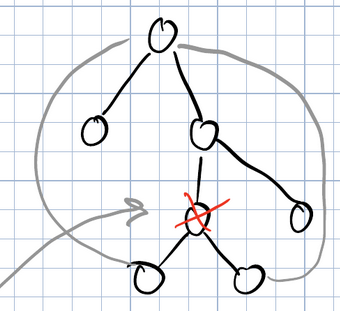
\includegraphics[width=\linewidth]{1}
	
	{\bf Процессы сироты} - процессы без родителей.
	
	Система продолжает сохранять иерархию процессов. Поэтому сироты усыновляются процессом, открывшим терминал ({\it cpid = 1}).
	
	{\it Но, как правило, все-таки есть посредники.}
	
	В системе всегда есть процессы с идентификатором 0 ({\bf процесс, запустивший систему}) и 1 ({\bf процесс, открывший терминал}) вне зависимости от количества терминалов (не нужно резервировать место под каждый терминал).
	
	Чтобы сироты не возникали, вызывается {\bf wait(\&status)} - блокирует процесс-предка до завершения процесса-потомка (процесс помечается ожидающим до завершения процесса-потомка).
	
	Такая ситуация с правами доступа к адресному пространству предка будет существовать в системе до тех пор, пока потомок не вызовет {\bf exec} или {\bf exit}. {\bf exit} завершает процесс, а {\bf exec} переводит процесс-потомок на адресное пространство программы, которое передано в качестве аргумента; в результате потомок начинает выполнять другую программу.
	
	Другими словами, в UNIX, чтобы запустить программу, нужно вызвать fork, и потомок должен вызвать exec (fork -> процесс -> exec -> программа).
	
	{\bf Момент:} Предки могут анализировать статус выполнения потомков.
	
	Кроме иерархии, система UNIX поддерживает {\bf группы процессов}. Процессы одной группы могут получать одни и те же сигналы.
	
	{\bf Сигналы} - важнейшее средство информирования о событиях в системе.
	
	{\bf Важнейшее событие - завершение процесса.}
	
	\section*{Прерывание INT 8h}
	
	<дописать>
\end{document}
